\documentclass{article} % For LaTeX2e
\usepackage{cos424,times}
\usepackage{hyperref}
\usepackage{url}
\usepackage{graphicx}
\usepackage{caption}
\usepackage{subcaption}
\usepackage{floatrow}
\usepackage{titlesec}
\usepackage[english]{babel}
\usepackage{blindtext}
\usepackage{wrapfig}
\setlength{\belowcaptionskip}{0pt}
\setlength{\abovecaptionskip}{3pt}
\setlength{\floatsep}{2pt}
\titlespacing*{\section}{-1pt}{0.2\baselineskip}{0.2\baselineskip}
\titlespacing*{\subsection}{-1pt}{0.2\baselineskip}{0.2\baselineskip}
\titlespacing*{\subsubsection}{-1pt}{0.2\baselineskip}{0.2\baselineskip}

\title{Audio Classification}


\author{
Julia Johnstone\\
Princeton University\\
\texttt{juliakj@princeton.edu} \\
\And
Zi Xiang Pan \\
Princeton University \\
\texttt{zpan@princeton.edu} \\
}

\newcommand{\fix}{\marginpar{FIX}}
\newcommand{\new}{\marginpar{NEW}}

\begin{document}

\maketitle

\begin{abstract}
This report concerns the problem of musical genre classification on the GZTAN dataset. We visualized the data before running a series of trials using different features and classifiers. Ultimately, we observed a maximum accuracy of 75.5\% using a soft-voting ensemble of classifiers. 
\end{abstract}

\section{Introduction}

In this report, we consider a common problem in musical machine learning: classification by genre. Specifically, we attempt to classify the well-known GTZAN dataset of a thousand 30-second snippets of songs divided evenly across the genres of blues, classical, country, disco, hip-hop, jazz, metal, pop, reggae, and rock.

The remainder of this paper describes some of the existing research genre classification, our methods of extracting and transforming features from the data, and the trials we ran to explore the relative effectiveness of various combinations of features and classifiers. We conclude by presenting and discussing the results of these trials.

\section{Related Work}

Machine learning has been used as a means of genre classification since 1997 when Carnegie Mellon researchers ran classifications on five-second song snippets\cite{Dannenberg}. 

\section{Methods}

As we approached this classification problem, we decided to begin by visualizing the data in order to gain some understanding of how the song samples differed across genre. Afterwards, we began running classification trials and comparing results. In these trials, we varied each of the following properties: features considered, classifiers used, and methods of combining the results of multiple classifiers.

\subsection{Data Visualization}
write this:
- what exactly were we graphing in the bar charts? just the raw data or fischer vectors?
- what we learned about the data

\subsection{Trial Design}
In order to compare the results of varying the features considered and classifiers used, we ran each classification trial in the same way. Specifically, we began by shuffling the data so that samples were no longer grouped by genre. We then used 10-fold cross validation to compute the error rate achieved. 

\subsection{Features}
Initially, we selected five features based on their promising performance in the literature: MFCC, Chroma, Energy, Spectral Flux, and HCDF. We then used the provided scripts to load the song samples in .mat format and extract the five features  from each sample. Because each feature considered is a frame-level feature and therefore high dimensional, we used the provided scripts to apply Fisher Vectors to each feature to generate descriptors before converting the results into .csv format. 

Once we had completed the extraction and quantization process, we experimented with varying the features considered in three ways.

\subsubsection{Experiment 1: Combinations of Features}
In this experiment, we ran trials for every combination of the five features encoded with Fisher Vectors. For each of eight classifiers considered, we collected the results of predicting based on each possible combination.

\subsubsection{Experiment 2: Reduction of MFCC}
In this experiment, we looked at the results of projecting the MFCC Fisher Vector down to lower dimension spaces and then running classifications. We ran trials using projections into 3 dimensions and 300 dimensions as features.

\subsubsection{Experiment 3: Using Raw Data}
The goal of this experiment was to compare the performance of Fisher Vector-generated descriptors with the performance of raw data.  Therefore, we ran trials with classifying on MFCC and HCDF in their FV and raw forms. 

\subsection{Classifiers}
write this
\subsubsection{Experiment 1: Vary Classifier}
write this

\subsection{Classifier Combinations}
Once we had collected the results achieved by single classifiers, we decided to try pooling the predictions of several classifiers into a single set of predictions. Therefore, we experimented with hard voting and soft voting using our best-performing classifiers.

\subsubsection{Experiment 1: Hard Voting}
In this experiment, we ran trials in which three classifiers - 5-Nearest Neighbors, Linear SVM, and Gaussian Naive Bayes - engaged in a hard vote to determine the final classification of a sample. This means that each classifier cast one vote per sample considered. Performance across each combination of FV features was considered.

\subsubsection{Experiment 2: Soft Voting} In this experiment, we conducted a soft vote of four classifiers: 5-Nearest Neighbors, Linear SVM, Gaussian Naive Bayes, and Random Forest with a forest of 50 trees. The best performing classifier, Linear SVM, was cast two votes while each of the others cast one. Again, performance across each combination of FV features was considered.










\section{Results}

\subsection{Preliminary Analysis}
\begin{figure}[h]
	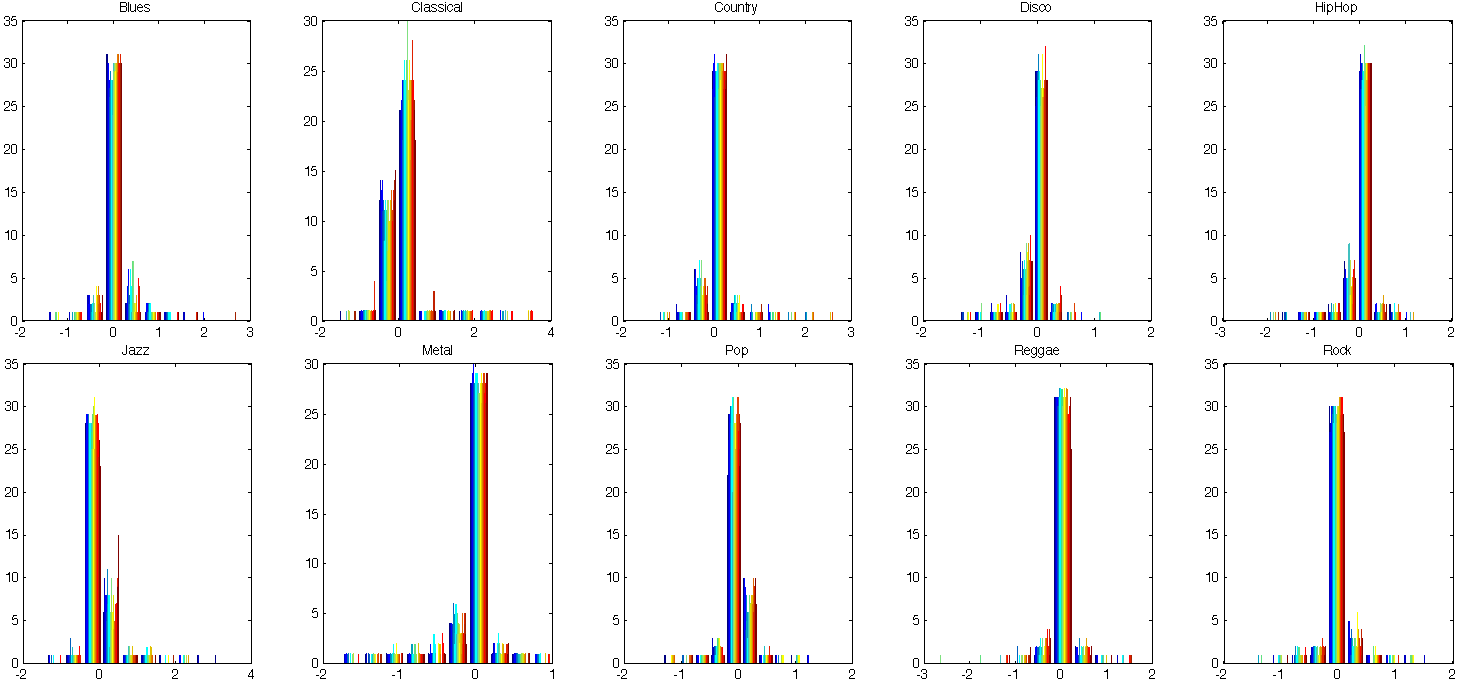
\includegraphics[width=\textwidth]{histgram_mfcc.png}
	\caption{Plots for time-averaged means of MFC coefficients for the 10 genres, every colored line represents one song}
\end{figure}
We see that the distribution of the means of MFC coefficients do indeed differ across genres, suggesting that MFCC is an informative feature for classification.

\begin{figure}[h]
	\begin{subfigure}[b]{0.49\textwidth}
		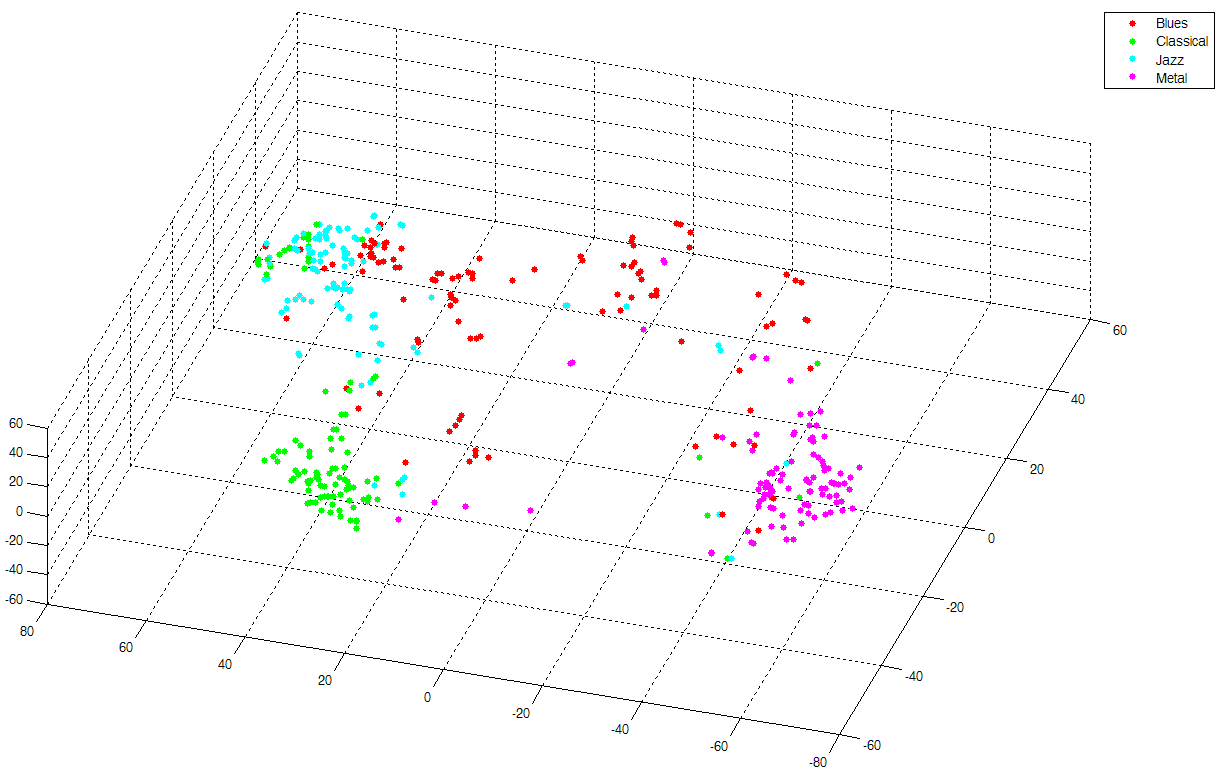
\includegraphics[width=\textwidth]{blues_classical_jazz_metal.png}
		\caption{t-sne subplots for Blues, Classical, Jazz, Metal showing clean separability}
		\label{fig:tsne1}
	\end{subfigure}
	\hfill
	\begin{subfigure}[b]{0.49\textwidth}
		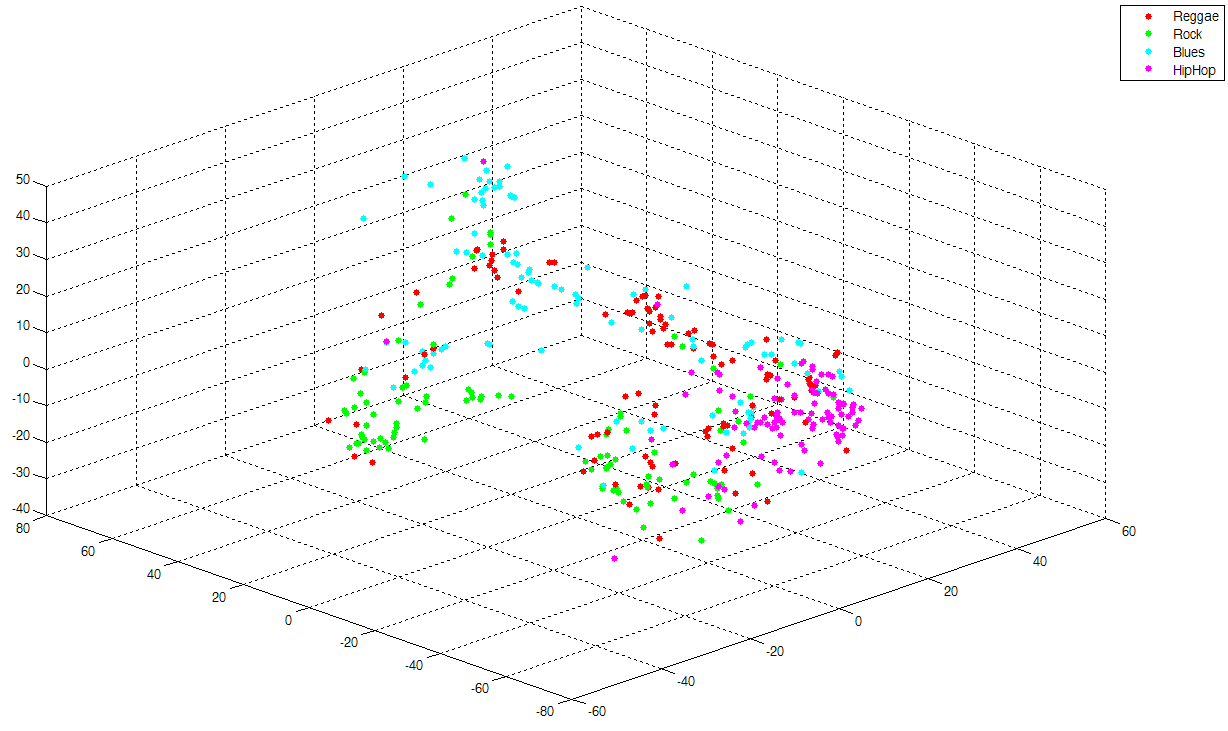
\includegraphics[width=\textwidth]{reggae_rock_blues_hiphop.png}
		\caption{same t-sne subplots for Reggae, Rock, Blues, Hip-Hop showing confusion}
		\label{fig:tsne2}
	\end{subfigure}
	\caption{t-sne plots in 3-D of a projection of 960-dimensional MFCC FV}
\end{figure}
We also see even in an extremely compressed 3-dimensional projection of the MFC data, t-sne is able to discern clear clusters of songs in each genre. This gives us a hint as to which genres are easily separated and which are easily confused.
\subsection{Combinations of features with different classifiers}
\begin{figure}[h]
	\begin{tabular}{|l|l|l|l|l|l|l|l|l|}
		\hline
					& KNN3  & KNN5  & SVM-Lin & SVM-RBF & GNB  & RF  & Softvote 2,3,5,6  & Hardvote 2,3,5 \\ \hline
		Min error   & 0.343 & 0.333 & 0.255  & 0.384  & 0.37 & 0.288  & 0.245  & 0.261 \\ \hline
		Feature set & \multicolumn{3}{l|}{\begin{tabular}[c]{@{}l@{}}MFCC\\ HCDF\end{tabular}} & MFCC    & \begin{tabular}[c]{@{}l@{}}MFCC\\ energy\end{tabular} & \begin{tabular}[c]{@{}l@{}}chroma\\ HCDF\end{tabular} & \begin{tabular}[c]{@{}l@{}}MFCC\\ chroma\\ brightness\end{tabular} & \begin{tabular}[c]{@{}l@{}}HCDF\\ brightness\end{tabular} \\ \hline
	\end{tabular}
	\caption{10-fold CV classification error rate for different classifiers and the features that performed the best, for full data table see appendix}
	\label{fig:classifiers}
\end{figure}
We see in \ref{fig:classifiers} that the feature set of MFCC, chroma and brightness performed with 0.245 error rate with a soft voting algorithm of KNN5, SVM(Linear kernel) Gaussian NB, and Random Forest.
\subsection{Fisher vectors vs PCA of raw timeframe data}
\begin{figure}[h]
	\floatbox[{\capbeside\thisfloatsetup{capbesideposition={right,top},capbesidewidth=4cm}}]{figure}[\FBwidth]
	{\caption{The error rates of two Feature FV against their raw data counterparts with two classifiers}\label{rawdata}}
	{
	\begin{tabular}{|l|l|l|}
		\hline
		& KNN3  & SVM-Lin \\ \hline
		MFCC FV         & 0.343 & 0.255   \\ \hline
		MFCC Raw data   & 0.461 & 0.396   \\ \hline
		Chroma FV       & 0.605 & 0.558   \\ \hline
		Chroma Raw data & 0.671 & 0.679   \\ \hline
	\end{tabular}
	}
\end{figure}
In \ref{rawdata} we see that the generated Fisher Vectors performs better than just a simple collection of raw data vectors


\section{Discussion and Conclusion}

\subsection{Confusion matrix}
\begin{wrapfigure}{l}{0.6\textwidth}
	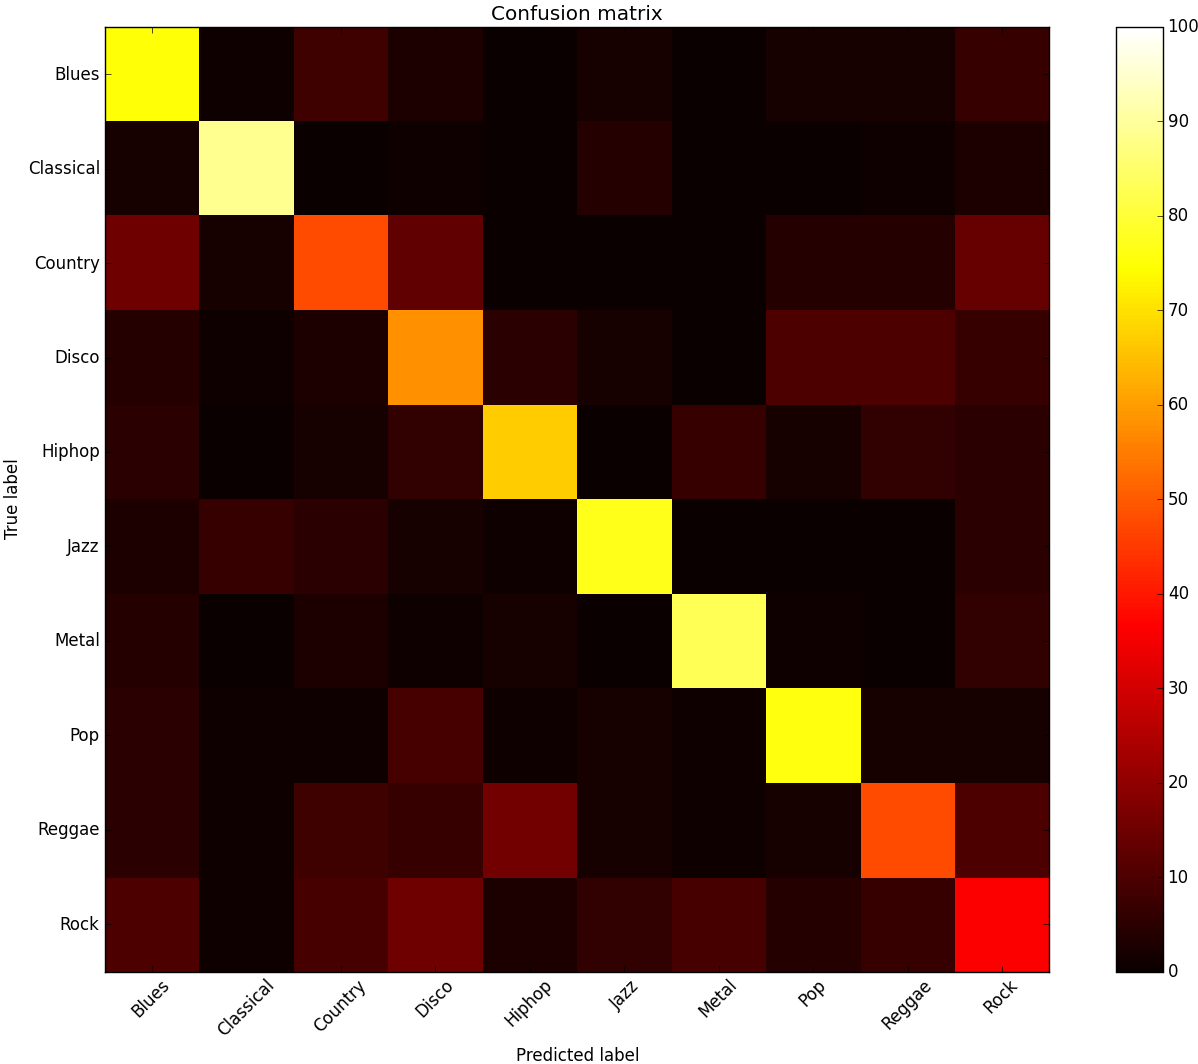
\includegraphics[width=\textwidth]{confusion_matrix.png}
	\caption{Confusion matrix of 10-fold CV predictions and true labels, white is 100\% accuracy, black is 0\%}
	\label{fig:confusion}
\end{wrapfigure}
The confusion matrix in figure \ref{fig:confusion} is built from MFCC+HCDF Fisher Vector feature set with KNN5 classifier. We see that Classical, Metal , Blues and Jazz are the best identified genres, with accuracy exceeding 70\%, this corroborates with our visualization in figure \ref{fig:tsne1} which showed clear clustering for those genres. Genre pairs with the most confusion are \{Reggae, Hip-Hop\}, \{Rock, Disco\}, \{Rock, Country\}, which also corroborates with our visualizations in figure \ref{fig:tsne2}. 
\subsection{Classifiers and features}
It is no surprise that the best single classifier before ensemble learning is linear SVM, because our underlying features are represented in Fisher Vectors, which lends itself to efficient linear classification.
The Fisher Kernel inherits advantages from both generative and discriminative models by building a kernel from a generative model (in this case GMM),  it characterizes a sample by its deviation from the model measured by computing the gradient of the sample log-likelihood with  respect  to  the  model  parameters.\cite{HAL}.


\subsubsection*{Acknowledgments}

We would like to acknowledge the creators of scikit-learn and its documentation. Being able to use opensource implementations of the methods and classifiers was extremely helpful. We would like to thank Professor Engelhardt and TAs who explained the project parameters. 

\bibliographystyle{acm}
\bibliography{ref}
\section{Appendix} \label{section:appendix}
\begin{figure}[V]
	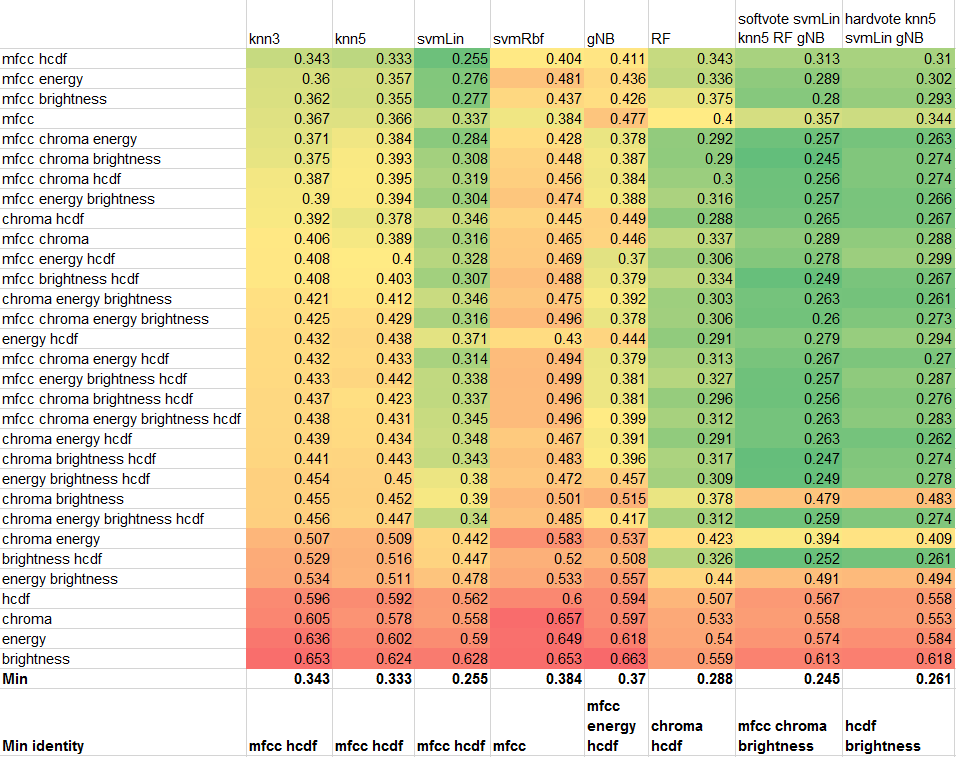
\includegraphics[width=\textwidth]{all_results.png}
	\caption{Full dataset of classification errors with different features and classifiers, greener is lower error}
	\label{fig:all_results}
\end{figure}
\begin{figure}[V]
	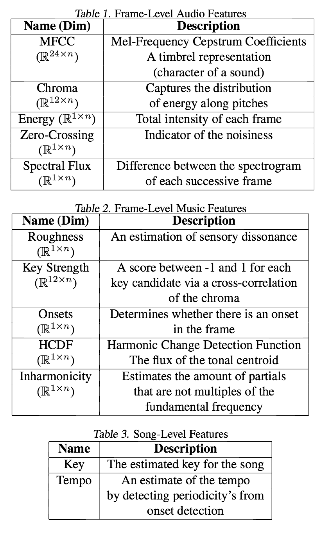
\includegraphics[width=0.6\textwidth]{features}
	\caption{This figure provides a description of various song features and was taken from the given sample paper. \cite{sample}.}
	\label{fig:featureSet}
\end{figure}
\end{document}
